\PassOptionsToPackage{unicode=true}{hyperref} % options for packages loaded elsewhere
\PassOptionsToPackage{hyphens}{url}
%
\documentclass[]{article}
\usepackage{lmodern}
\usepackage{amssymb,amsmath}
\usepackage{ifxetex,ifluatex}
\usepackage{fixltx2e} % provides \textsubscript
\ifnum 0\ifxetex 1\fi\ifluatex 1\fi=0 % if pdftex
  \usepackage[T1]{fontenc}
  \usepackage[utf8]{inputenc}
  \usepackage{textcomp} % provides euro and other symbols
\else % if luatex or xelatex
  \usepackage{unicode-math}
  \defaultfontfeatures{Ligatures=TeX,Scale=MatchLowercase}
\fi
% use upquote if available, for straight quotes in verbatim environments
\IfFileExists{upquote.sty}{\usepackage{upquote}}{}
% use microtype if available
\IfFileExists{microtype.sty}{%
\usepackage[]{microtype}
\UseMicrotypeSet[protrusion]{basicmath} % disable protrusion for tt fonts
}{}
\IfFileExists{parskip.sty}{%
\usepackage{parskip}
}{% else
\setlength{\parindent}{0pt}
\setlength{\parskip}{6pt plus 2pt minus 1pt}
}
\usepackage{hyperref}
\hypersetup{
            pdftitle={Project 2: Modeling, Testing, and Predicting Headache Status},
            pdfauthor={Mikayla Oldham - mio289},
            pdfborder={0 0 0},
            breaklinks=true}
\urlstyle{same}  % don't use monospace font for urls
\usepackage[margin=1in]{geometry}
\usepackage{color}
\usepackage{fancyvrb}
\newcommand{\VerbBar}{|}
\newcommand{\VERB}{\Verb[commandchars=\\\{\}]}
\DefineVerbatimEnvironment{Highlighting}{Verbatim}{commandchars=\\\{\}}
% Add ',fontsize=\small' for more characters per line
\usepackage{framed}
\definecolor{shadecolor}{RGB}{248,248,248}
\newenvironment{Shaded}{\begin{snugshade}}{\end{snugshade}}
\newcommand{\AlertTok}[1]{\textcolor[rgb]{0.94,0.16,0.16}{#1}}
\newcommand{\AnnotationTok}[1]{\textcolor[rgb]{0.56,0.35,0.01}{\textbf{\textit{#1}}}}
\newcommand{\AttributeTok}[1]{\textcolor[rgb]{0.77,0.63,0.00}{#1}}
\newcommand{\BaseNTok}[1]{\textcolor[rgb]{0.00,0.00,0.81}{#1}}
\newcommand{\BuiltInTok}[1]{#1}
\newcommand{\CharTok}[1]{\textcolor[rgb]{0.31,0.60,0.02}{#1}}
\newcommand{\CommentTok}[1]{\textcolor[rgb]{0.56,0.35,0.01}{\textit{#1}}}
\newcommand{\CommentVarTok}[1]{\textcolor[rgb]{0.56,0.35,0.01}{\textbf{\textit{#1}}}}
\newcommand{\ConstantTok}[1]{\textcolor[rgb]{0.00,0.00,0.00}{#1}}
\newcommand{\ControlFlowTok}[1]{\textcolor[rgb]{0.13,0.29,0.53}{\textbf{#1}}}
\newcommand{\DataTypeTok}[1]{\textcolor[rgb]{0.13,0.29,0.53}{#1}}
\newcommand{\DecValTok}[1]{\textcolor[rgb]{0.00,0.00,0.81}{#1}}
\newcommand{\DocumentationTok}[1]{\textcolor[rgb]{0.56,0.35,0.01}{\textbf{\textit{#1}}}}
\newcommand{\ErrorTok}[1]{\textcolor[rgb]{0.64,0.00,0.00}{\textbf{#1}}}
\newcommand{\ExtensionTok}[1]{#1}
\newcommand{\FloatTok}[1]{\textcolor[rgb]{0.00,0.00,0.81}{#1}}
\newcommand{\FunctionTok}[1]{\textcolor[rgb]{0.00,0.00,0.00}{#1}}
\newcommand{\ImportTok}[1]{#1}
\newcommand{\InformationTok}[1]{\textcolor[rgb]{0.56,0.35,0.01}{\textbf{\textit{#1}}}}
\newcommand{\KeywordTok}[1]{\textcolor[rgb]{0.13,0.29,0.53}{\textbf{#1}}}
\newcommand{\NormalTok}[1]{#1}
\newcommand{\OperatorTok}[1]{\textcolor[rgb]{0.81,0.36,0.00}{\textbf{#1}}}
\newcommand{\OtherTok}[1]{\textcolor[rgb]{0.56,0.35,0.01}{#1}}
\newcommand{\PreprocessorTok}[1]{\textcolor[rgb]{0.56,0.35,0.01}{\textit{#1}}}
\newcommand{\RegionMarkerTok}[1]{#1}
\newcommand{\SpecialCharTok}[1]{\textcolor[rgb]{0.00,0.00,0.00}{#1}}
\newcommand{\SpecialStringTok}[1]{\textcolor[rgb]{0.31,0.60,0.02}{#1}}
\newcommand{\StringTok}[1]{\textcolor[rgb]{0.31,0.60,0.02}{#1}}
\newcommand{\VariableTok}[1]{\textcolor[rgb]{0.00,0.00,0.00}{#1}}
\newcommand{\VerbatimStringTok}[1]{\textcolor[rgb]{0.31,0.60,0.02}{#1}}
\newcommand{\WarningTok}[1]{\textcolor[rgb]{0.56,0.35,0.01}{\textbf{\textit{#1}}}}
\usepackage{graphicx,grffile}
\makeatletter
\def\maxwidth{\ifdim\Gin@nat@width>\linewidth\linewidth\else\Gin@nat@width\fi}
\def\maxheight{\ifdim\Gin@nat@height>\textheight\textheight\else\Gin@nat@height\fi}
\makeatother
% Scale images if necessary, so that they will not overflow the page
% margins by default, and it is still possible to overwrite the defaults
% using explicit options in \includegraphics[width, height, ...]{}
\setkeys{Gin}{width=\maxwidth,height=\maxheight,keepaspectratio}
\setlength{\emergencystretch}{3em}  % prevent overfull lines
\providecommand{\tightlist}{%
  \setlength{\itemsep}{0pt}\setlength{\parskip}{0pt}}
\setcounter{secnumdepth}{0}
% Redefines (sub)paragraphs to behave more like sections
\ifx\paragraph\undefined\else
\let\oldparagraph\paragraph
\renewcommand{\paragraph}[1]{\oldparagraph{#1}\mbox{}}
\fi
\ifx\subparagraph\undefined\else
\let\oldsubparagraph\subparagraph
\renewcommand{\subparagraph}[1]{\oldsubparagraph{#1}\mbox{}}
\fi

% set default figure placement to htbp
\makeatletter
\def\fps@figure{htbp}
\makeatother


\title{Project 2: Modeling, Testing, and Predicting Headache Status}
\author{Mikayla Oldham - mio289}
\date{}

\begin{document}
\maketitle

\#\#\#Introduction to the data: The following data was pulled from a
study by Tammy Kostecki-Dillon that was conducted on patients who
suffered chronic headaches. The \textbf{numeric variables} include
``id'' which identifies each patient, ``dos'' which measures the time in
days since the patient began participation in the study, ``time'' which
measures the time in days since the onset of treatment during the study
(with negative values representing the number of days before the onset
of treatment), ``age'' which measures the age in years of the patient,
and ``airq'' which measures the air quality index for that day with a
higher air index representing worse air quality and a lower index
representing better air quality. The first \textbf{categorical variable}
is ``hatype'' which identifies the type of headache as being ``aura''
for a aura headache, ``non-aura'' for a headache that does not contain
aura symptoms, or ``mixed'' for a headache that demonstrates some
symptoms of a normal headache and some symptoms of an aura headache. The
next categorical variable is ``medication'' which identifies the level
of treatment through whether it is being ``continued'', ``reduced'', or
``none'' for stopped treatment. The last categorical variables are
``headache'' which identifies a day with a headahe as ``yes'' and a day
without a headache as ``no'', while ``sex'' represents whether the
patient is ``male'' or ``female''. There are a total of \textbf{4152
observations} in this data set.

As someone who frequently experiences symptoms of auras prior to a
migraine, I found this data set to be really interesting! I was eager to
see if there were any aspects that might predict the onset of auras, and
the variables in the data provided a great opportunity to explore this
through regressions. A glimpse of the data is shown below:

\begin{Shaded}
\begin{Highlighting}[]
\NormalTok{headache <-}\StringTok{ }\KeywordTok{read.csv}\NormalTok{(}\StringTok{"https://vincentarelbundock.github.io/Rdatasets/csv/carData/KosteckiDillon.csv"}\NormalTok{)}
\NormalTok{headache <-}\StringTok{ }\NormalTok{headache }\OperatorTok\StringTok{ }\KeywordTok{select}\NormalTok{(}\OperatorTok{-}\NormalTok{X)}
\KeywordTok{head}\NormalTok{(headache)}
\end{Highlighting}
\end{Shaded}

\begin{verbatim}
##   id time dos hatype age airq medication headache    sex
## 1  1  -11 753   Aura  30    9 continuing      yes female
## 2  1  -10 754   Aura  30    7 continuing      yes female
## 3  1   -9 755   Aura  30   10 continuing      yes female
## 4  1   -8 756   Aura  30   13 continuing      yes female
## 5  1   -7 757   Aura  30   18 continuing      yes female
## 6  1   -6 758   Aura  30   19 continuing      yes female
\end{verbatim}

\#\#\#MANOVA \& ANOVA The following MANOVA test was conducted to
determine if any considered numeric variable, age or airquality, had
significantly different mean values for the different types of
headaches: aura, non-aura, or mixed. This test could be important for
further analysis testing if certain demographic factors, such as age or
airquality in the city of residence, can cause people to have a
predisposition for certain types of headaches.

First, the assumptions were checked:

\begin{itemize}
\tightlist
\item
  The tested data was from a \textbf{random sample} and the observations
  were \textbf{independent} \(\checkmark\)
\item
  \textbf{Multivariate Normality}:
\end{itemize}

\begin{Shaded}
\begin{Highlighting}[]
\KeywordTok{ggplot}\NormalTok{(headache, }\KeywordTok{aes}\NormalTok{(}\DataTypeTok{x =}\NormalTok{ age, }\DataTypeTok{y =}\NormalTok{ airq)) }\OperatorTok{+}\StringTok{ }
\StringTok{  }\KeywordTok{geom_point}\NormalTok{(}\DataTypeTok{alpha=}\NormalTok{.}\DecValTok{5}\NormalTok{) }\OperatorTok{+}\StringTok{ }\KeywordTok{geom_density_2d}\NormalTok{(}\DataTypeTok{h=}\DecValTok{2}\NormalTok{) }\OperatorTok{+}
\StringTok{  }\KeywordTok{coord_fixed}\NormalTok{() }\OperatorTok{+}\StringTok{ }\KeywordTok{facet_wrap}\NormalTok{(}\OperatorTok{~}\NormalTok{hatype)}
\end{Highlighting}
\end{Shaded}

\begin{center}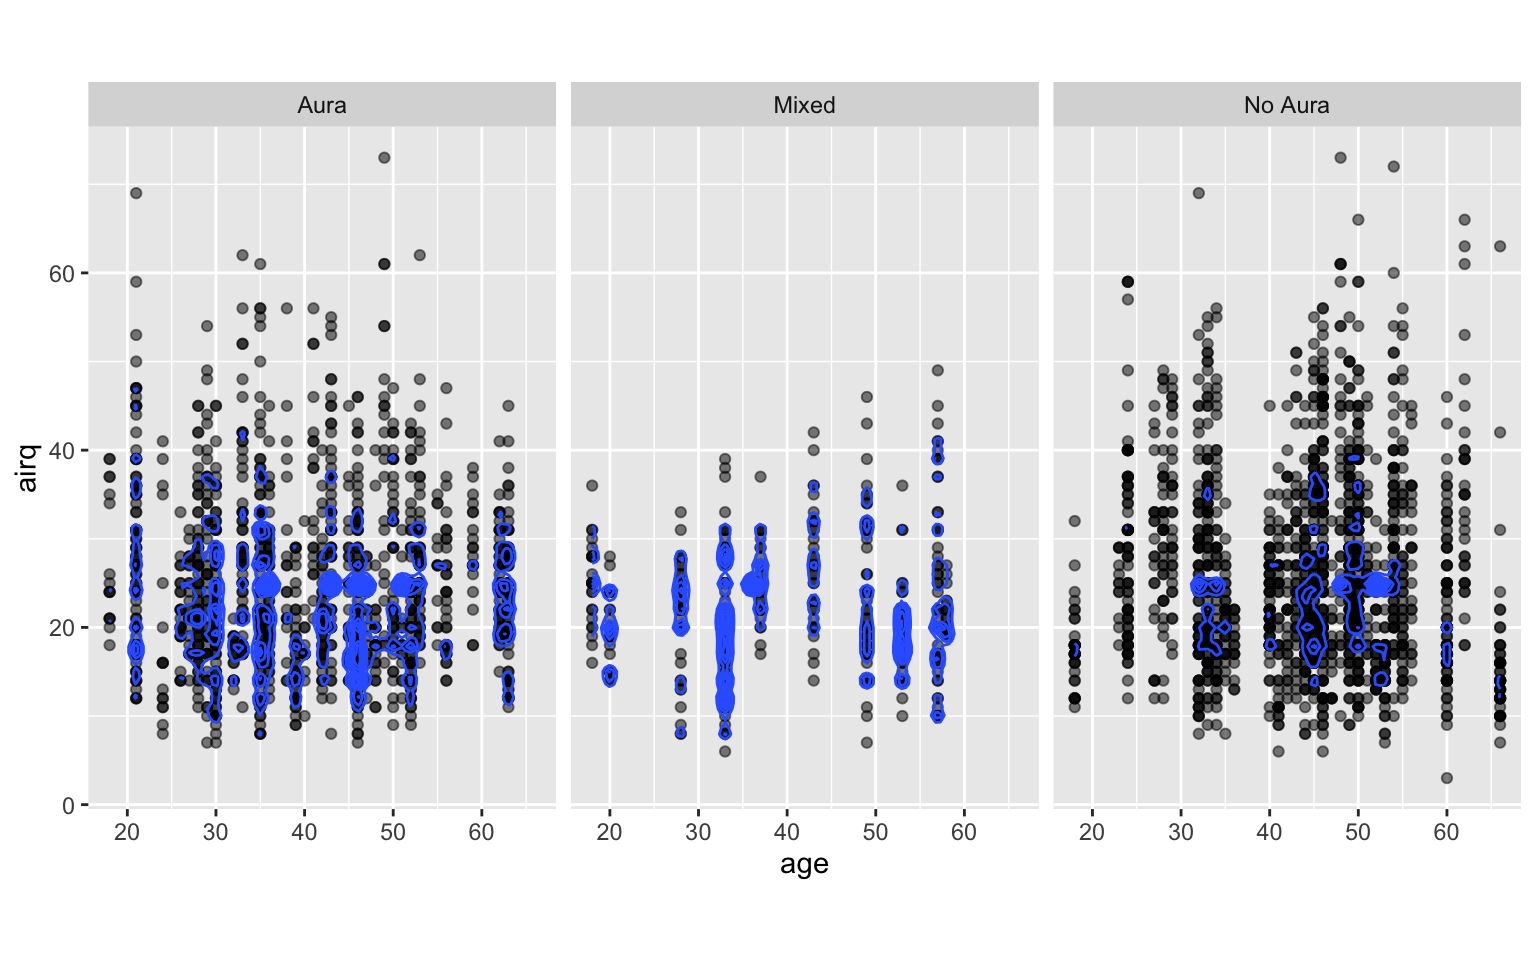
\includegraphics{project2final_files/figure-latex/unnamed-chunk-2-1} \end{center}

Based on these plots, there is no clear normality of the data in each
group. Therefore, the assumption of multivariate normality is not met
and we proceed with caution.

\begin{itemize}
\tightlist
\item
  \textbf{Homogeneity of within-group covariance matrices}:
\end{itemize}

\begin{Shaded}
\begin{Highlighting}[]
\NormalTok{covariance <-}\StringTok{ }\NormalTok{headache }\OperatorTok\StringTok{ }\KeywordTok{group_by}\NormalTok{(hatype) }\OperatorTok\StringTok{ }\KeywordTok{do}\NormalTok{(}\DataTypeTok{covs=}\KeywordTok{cov}\NormalTok{(.[}\DecValTok{5}\OperatorTok{:}\DecValTok{6}\NormalTok{]))}
\ControlFlowTok{for}\NormalTok{(i }\ControlFlowTok{in} \DecValTok{1}\OperatorTok{:}\DecValTok{3}\NormalTok{)\{}\KeywordTok{print}\NormalTok{(}\KeywordTok{as.character}\NormalTok{(covariance}\OperatorTok{$}\NormalTok{hatype[i]))}
\KeywordTok{print}\NormalTok{(covariance}\OperatorTok{$}\NormalTok{covs[i])\}}
\end{Highlighting}
\end{Shaded}

\begin{verbatim}
## [1] "Aura"
## [[1]]
##             age      airq
## age  129.408036 -3.205749
## airq  -3.205749 83.063081
## 
## [1] "Mixed"
## [[1]]
##             age      airq
## age  154.518926  5.285457
## airq   5.285457 50.556670
## 
## [1] "No Aura"
## [[1]]
##             age       airq
## age  108.879813  -4.513002
## airq  -4.513002 103.442276
\end{verbatim}

The covariance among all headache types appear to differ. The
homogeneity of covariance assumption is not met so again, we proceed
with caution.

After checking assumptions, the test was conducted.

\begin{itemize}
\item
  Ho: For both age and airquality, the means of the headache type groups
  are equal.
\item
  HA: For atleast one of the response variables, either age, airquality,
  or both, atleast 1 of the headache type means is different than the
  others.
\end{itemize}

\begin{Shaded}
\begin{Highlighting}[]
\NormalTok{man <-}\StringTok{ }\KeywordTok{manova}\NormalTok{(}\KeywordTok{cbind}\NormalTok{(age, airq) }\OperatorTok{~}\StringTok{ }\NormalTok{hatype, }\DataTypeTok{data=}\NormalTok{headache)}
\KeywordTok{summary}\NormalTok{(man)}
\end{Highlighting}
\end{Shaded}

\begin{verbatim}
## Df Pillai approx F num Df den Df Pr(>F)
## hatype 2 0.040322 42.684 4 8298 < 2.2e-16 ***
## Residuals 4149
## ---
## Signif. codes: 0 '***' 0.001 '**' 0.01 '*' 0.05 '.' 0.1
' ' 1
\end{verbatim}

Based on these results, there is a significant difference among the
headache types for atleast one of the dependent variables
(p\textless{}0.001).

Since the MANOVA results were significant, \textbf{univariate ANOVA
tests} were run to see which dependent variable, age or airquality, had
a significantly different mean value for atleast one of the headache
types.

\begin{Shaded}
\begin{Highlighting}[]
\KeywordTok{summary.aov}\NormalTok{(man) }
\end{Highlighting}
\end{Shaded}

\begin{verbatim}
## Response age :
## Df Sum Sq Mean Sq F value Pr(>F)
## hatype 2 13181 6590.3 53.864 < 2.2e-16 ***
## Residuals 4149 507637 122.4
## ---
## Signif. codes: 0 '***' 0.001 '**' 0.01 '*' 0.05 '.' 0.1
' ' 1
##
## Response airq :
## Df Sum Sq Mean Sq F value Pr(>F)
## hatype 2 5516 2758.13 30.909 4.738e-14 ***
## Residuals 4149 370238 89.24
## ---
## Signif. codes: 0 '***' 0.001 '**' 0.01 '*' 0.05 '.' 0.1
' ' 1
\end{verbatim}

The ANOVA results show that both age (p\textless{}.001) and airquality
(p\textless{}.001) have significant mean differences for atleast one of
the headache types. This was prior to adjusting the significance level
based on the type 1 error rate, which will be discussed further below.

Since the ANOVA results were found to be significant, \textbf{post-hoc
analysis tests} were conducted to determine which headache type had
differing means for the age variable and for the airquality variable.

\begin{Shaded}
\begin{Highlighting}[]
\NormalTok{headache }\OperatorTok\StringTok{ }\KeywordTok{group_by}\NormalTok{(hatype) }\OperatorTok\StringTok{ }\KeywordTok{summarize}\NormalTok{(}\KeywordTok{mean}\NormalTok{(age), }\KeywordTok{mean}\NormalTok{(airq))}
\end{Highlighting}
\end{Shaded}

\begin{verbatim}
## # A tibble: 3 x 3
##   hatype  `mean(age)` `mean(airq)`
##   <chr>         <dbl>        <dbl>
## 1 Aura           40.9         24.3
## 2 Mixed          40.0         22.4
## 3 No Aura        44.2         25.9
\end{verbatim}

\begin{Shaded}
\begin{Highlighting}[]
\KeywordTok{pairwise.t.test}\NormalTok{(headache}\OperatorTok{$}\NormalTok{airq, headache}\OperatorTok{$}\NormalTok{hatype, }\DataTypeTok{p.adj=}\StringTok{"none"}\NormalTok{)}
\end{Highlighting}
\end{Shaded}

\begin{verbatim}
## 
##  Pairwise comparisons using t tests with pooled SD 
## 
## data:  headache$airq and headache$hatype 
## 
##         Aura    Mixed  
## Mixed   0.00012 -      
## No Aura 2.6e-07 7.6e-13
## 
## P value adjustment method: none
\end{verbatim}

\begin{Shaded}
\begin{Highlighting}[]
\KeywordTok{pairwise.t.test}\NormalTok{(headache}\OperatorTok{$}\NormalTok{age, headache}\OperatorTok{$}\NormalTok{hatype, }\DataTypeTok{p.adj=}\StringTok{"none"}\NormalTok{)}
\end{Highlighting}
\end{Shaded}

\begin{verbatim}
## 
##  Pairwise comparisons using t tests with pooled SD 
## 
## data:  headache$age and headache$hatype 
## 
##         Aura    Mixed  
## Mixed   0.12    -      
## No Aura < 2e-16 1.9e-13
## 
## P value adjustment method: none
\end{verbatim}

According to the pairwise comparisons, all three headache types had
significantly different mean values of airquality (p\textless{}0.001).
For the age variable, it was found that all headache types had different
mean values (p\textless{}.001) except for when comparing age values for
``aura'' headaches and ``mixed'' headaches (p=.12). Again, these
significance comparison values were based on alpha=0.05, but adjusted
significant levels are discussed below. The conclusion that ``aura'' and
``mixed'' groups do not have significantly different mean ages is
consistent with the average values seen in the table above, as these two
groups had average values both at about 40 years, while the ``no aura''
group had a higher average age of about 44 years. Likewise, the
airquality conclusion of all different averages is supported by the fact
that the ``no aura'' group had an average airquality of almost 26, the
``aura'' group had an average airquality of about 24, and the ``mixed''
group has an average airquality of about 22.

Next, the \textbf{probability of Type I errors} was recalculated because
there were 9 hypothesis tests total (1 MANOVA, 2 ANOVA, and 6 pairwise
t-tests). Because the probability of executing a Type I error increases
with each comparison, and there were 9 tests conducted above, the
probability was corrected by:

\begin{Shaded}
\begin{Highlighting}[]
\CommentTok{#P(type l error):}
\DecValTok{1}\OperatorTok{-}\NormalTok{((.}\DecValTok{95}\NormalTok{)}\OperatorTok{^}\DecValTok{9}\NormalTok{)}
\end{Highlighting}
\end{Shaded}

\begin{verbatim}
## [1] 0.3697506
\end{verbatim}

The corrected probablity of a Type 1 error, based on the 9 hypothesis
tests that were conducted, ends up being 0.3698. This is higher than the
normal error rate we see with one test, which is 0.05, because each
individual test has the 0.05 error rate.

To account for this increase in probability of Type 1 error due to
repeated hypothesis tests, the \textbf{Bonferroni correction} was
applied. The new alpha-p-value used for significance comparisons was
calculated by:

\begin{Shaded}
\begin{Highlighting}[]
\CommentTok{#Bonferroni corrected alpha:}
\FloatTok{.05}\OperatorTok{/}\DecValTok{9}
\end{Highlighting}
\end{Shaded}

\begin{verbatim}
## [1] 0.005555556
\end{verbatim}

By dividing the alpha value for one test by the number of tests
conducted, the new alpha value used for comparisons is .00556. This
means that by comparing test p-values to this corrected alpha-p-value,
we keep the overall Type I error rate at .05. When using this Bonferroni
corrected alpha value for the tests conducted above, all results that
were considered significant before remain significant because they are
all less than alpha=.00556; average age differed between all headache
types except for ``aura'' and ``mixed'', while average airquality
differed between all headache types.

*It is important to note that though we found significant differences in
the means among headache types, the assumptions were not all initially
met. Therefore, the interpretations of these results are not necessarily
reliable. For example, because the covariances were not found to be
homogenous across groups, the mean differeneces could be due to
inconsistent variance and not necessarily significant differences due to
group type.

\#\#\#Randomization Test A randomization test was performed to simulate
the paired t-test in a different way. This time, we focused on
airquality and presence of headache to see if airquality differed at
times when someone experienced a headache as opposed to when they did
not experience a headache. These results could lead to studies that
determine if airquality has an effect on headache onset.

First, the mean differences in airquality for the different headache
responses were calculated. Then, responses of air quality were randomly
assigned to headache presence and a \textbf{null distribution} was
created.

\begin{Shaded}
\begin{Highlighting}[]
\NormalTok{real <-}\StringTok{ }\NormalTok{(}\KeywordTok{mean}\NormalTok{(headache[headache}\OperatorTok{$}\NormalTok{headache}\OperatorTok{==}\StringTok{"yes"}\NormalTok{,]}\OperatorTok{$}\NormalTok{airq) }\OperatorTok{-}\StringTok{ }
\StringTok{           }\KeywordTok{mean}\NormalTok{(headache[headache}\OperatorTok{$}\NormalTok{headache}\OperatorTok{==}\StringTok{"no"}\NormalTok{,]}\OperatorTok{$}\NormalTok{airq))}
\NormalTok{real}
\end{Highlighting}
\end{Shaded}

\begin{verbatim}
## [1] 0.2849134
\end{verbatim}

\begin{Shaded}
\begin{Highlighting}[]
\NormalTok{random <-}\StringTok{ }\KeywordTok{vector}\NormalTok{()}
\ControlFlowTok{for}\NormalTok{(i }\ControlFlowTok{in} \DecValTok{1}\OperatorTok{:}\DecValTok{5000}\NormalTok{)\{}
\NormalTok{  mixed <-}\StringTok{ }\KeywordTok{data.frame}\NormalTok{(}\DataTypeTok{airq=}\KeywordTok{sample}\NormalTok{(headache}\OperatorTok{$}\NormalTok{airq), }\DataTypeTok{presence=}\NormalTok{headache}\OperatorTok{$}\NormalTok{headache)}
\NormalTok{  random[i] <-}\StringTok{ }\NormalTok{(}\KeywordTok{mean}\NormalTok{(mixed[mixed}\OperatorTok{$}\NormalTok{presence}\OperatorTok{==}\StringTok{"yes"}\NormalTok{,]}\OperatorTok{$}\NormalTok{airq) }\OperatorTok{-}
\StringTok{                  }\KeywordTok{mean}\NormalTok{(mixed[mixed}\OperatorTok{$}\NormalTok{presence}\OperatorTok{==}\StringTok{"no"}\NormalTok{,]}\OperatorTok{$}\NormalTok{airq))\}}
\NormalTok{\{}\KeywordTok{hist}\NormalTok{(random, }\DataTypeTok{main=}\StringTok{"Null Distribution"}\NormalTok{, }\DataTypeTok{xlab=}\StringTok{"Difference in Airquality"}\NormalTok{); }
  \KeywordTok{abline}\NormalTok{(}\DataTypeTok{v =} \FloatTok{0.2849134}\NormalTok{, }\DataTypeTok{col=}\StringTok{"red"}\NormalTok{); }\KeywordTok{abline}\NormalTok{(}\DataTypeTok{v =} \FloatTok{-0.2849134}\NormalTok{, }\DataTypeTok{col=}\StringTok{"red"}\NormalTok{)\}}
\end{Highlighting}
\end{Shaded}

\begin{center}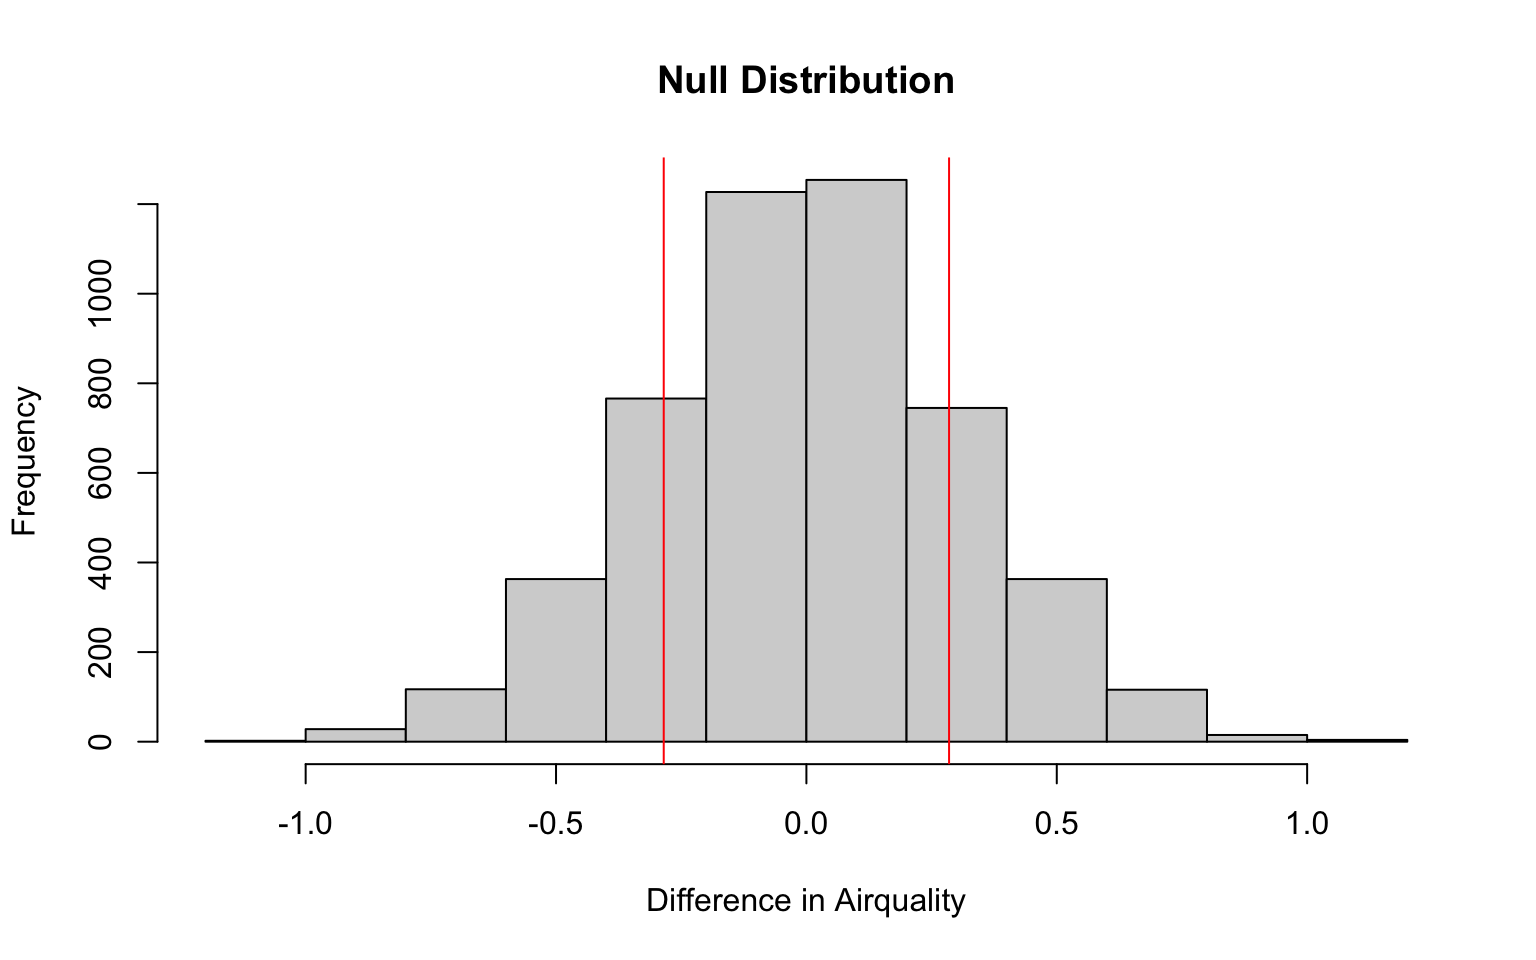
\includegraphics{project2final_files/figure-latex/unnamed-chunk-9-1} \end{center}

From the created null distribution, the hypotheses were tested by
comparing the actual mean difference to the null distribution.

\begin{itemize}
\item
  Ho: Airquality does not differ significantly for days that headaches
  were experienced versus days that headaches were not experienced.
\item
  HA: Airquality differs significantly for days that headaches were
  experienced versus days that headaches were not experienced.
\end{itemize}

The p-value was then calculated. This value tells the probability that
the real mean difference is observed under the null distribution which
assumes no association between airquality and headache presence.

\begin{Shaded}
\begin{Highlighting}[]
\KeywordTok{mean}\NormalTok{(random }\OperatorTok{>}\StringTok{ }\FloatTok{0.2849134} \OperatorTok{|}\StringTok{ }\NormalTok{random }\OperatorTok{<}\StringTok{ }\FloatTok{-0.2849134}\NormalTok{)}
\end{Highlighting}
\end{Shaded}

\begin{verbatim}
## [1] 0.3478
\end{verbatim}

The p-value was calculated to be 0.3498, which means there is almost a
35\% chance that we would observe the real mean difference of air
quality when there is no association between air quality and headache
presence. This value is much larger than alpha=.05, therefore we fail to
reject the null hypothesis and must assume that airquality does not
differ significantly for days that headaches were experienced versus
days that headaches were not experienced.

\#\#\#Linear Regression A linear regression was run to determine the
effects of sex, age, and their interaction on the proportion of days
that a participant experienced a headache. Predicting the occurance of a
headache from age and sex might help see if certain people are more
likely to experience headaches than others. In order to do this, a new
variable called ``prop\_head'' was created that represented the
proportion of days in the study that the individual experienced a
headache. The variable of ``age'' was also mean centered, represented by
``age\_c''. Then, the regression was run with these new variables.

\begin{Shaded}
\begin{Highlighting}[]
\NormalTok{headache2 <-}\StringTok{ }\NormalTok{headache }\OperatorTok\StringTok{ }\KeywordTok{select}\NormalTok{(id, age, sex, headache) }\OperatorTok\StringTok{ }
\StringTok{  }\KeywordTok{group_by}\NormalTok{(id) }\OperatorTok\StringTok{ }\KeywordTok{mutate}\NormalTok{(}\DataTypeTok{prop_head=}\KeywordTok{mean}\NormalTok{(headache}\OperatorTok{==}\StringTok{"yes"}\NormalTok{)) }\OperatorTok
\StringTok{  }\KeywordTok{select}\NormalTok{(}\OperatorTok{-}\NormalTok{headache) }\OperatorTok\StringTok{ }\KeywordTok{distinct}\NormalTok{()}
\NormalTok{headache2}\OperatorTok{$}\NormalTok{age_c <-}\StringTok{ }\NormalTok{headache2}\OperatorTok{$}\NormalTok{age }\OperatorTok{-}\StringTok{ }\KeywordTok{mean}\NormalTok{(headache2}\OperatorTok{$}\NormalTok{age)}

\NormalTok{fit1 <-}\StringTok{ }\KeywordTok{lm}\NormalTok{(prop_head}\OperatorTok{~}\NormalTok{age_c}\OperatorTok{+}\NormalTok{sex}\OperatorTok{+}\NormalTok{age_c}\OperatorTok{*}\NormalTok{sex, }\DataTypeTok{data=}\NormalTok{headache2)}
\KeywordTok{summary}\NormalTok{(fit1)}
\end{Highlighting}
\end{Shaded}

\begin{verbatim}
##
## Call:
## lm(formula = prop_head ~ age_c + sex + age_c * sex, data
= headache2)
##
## Residuals:
## Min 1Q Median 3Q Max
## -0.67929 -0.19286 0.03694 0.21243 0.39613
##
## Coefficients:
## Estimate Std. Error t value Pr(>|t|)
## (Intercept) 0.646629 0.025216 25.643 <2e-16 ***
## age_c -0.002155 0.002263 -0.952 0.343
## sexmale -0.011201 0.066021 -0.170 0.866
## age_c:sexmale -0.005369 0.005458 -0.984 0.327
## ---
## Signif. codes: 0 '***' 0.001 '**' 0.01 '*' 0.05 '.' 0.1
' ' 1
##
## Residual standard error: 0.2679 on 129 degrees of
freedom
## Multiple R-squared: 0.02575, Adjusted R-squared:
0.003097
## F-statistic: 1.137 on 3 and 129 DF, p-value: 0.3368
\end{verbatim}

The summary of the linear regression reveals the coefficients, which can
be interpreted as: ``intercept'' shows that for a female of average age,
the proportion of days that headaches are experienced is predicted to be
.646629; ``age\_c'' states that for every 1 year age increase, the
predicted proportion of headache days decreases by .002155; ``sexmale''
shows that for a person of average age, their proportion of headache
days is predited to decrease by .011201 if they are male;
``age\_c:sexmale'' shows that for males, a 1 year increase in age
decreases the predicted proportion of headache days by .005369 more than
for females.

This regression can be visualized by:

\begin{Shaded}
\begin{Highlighting}[]
\KeywordTok{ggplot}\NormalTok{(fit1, }\KeywordTok{aes}\NormalTok{(age_c, prop_head, }\DataTypeTok{color=}\NormalTok{sex)) }\OperatorTok{+}\StringTok{ }\KeywordTok{geom_point}\NormalTok{() }\OperatorTok{+}\StringTok{ }
\StringTok{  }\KeywordTok{geom_smooth}\NormalTok{(}\DataTypeTok{method=}\StringTok{'lm'}\NormalTok{, }\DataTypeTok{se=}\NormalTok{F) }\OperatorTok{+}\StringTok{ }
\StringTok{  }\KeywordTok{ggtitle}\NormalTok{(}\StringTok{"Proportion of Headache Days by Age and Sex"}\NormalTok{)}
\end{Highlighting}
\end{Shaded}

\begin{center}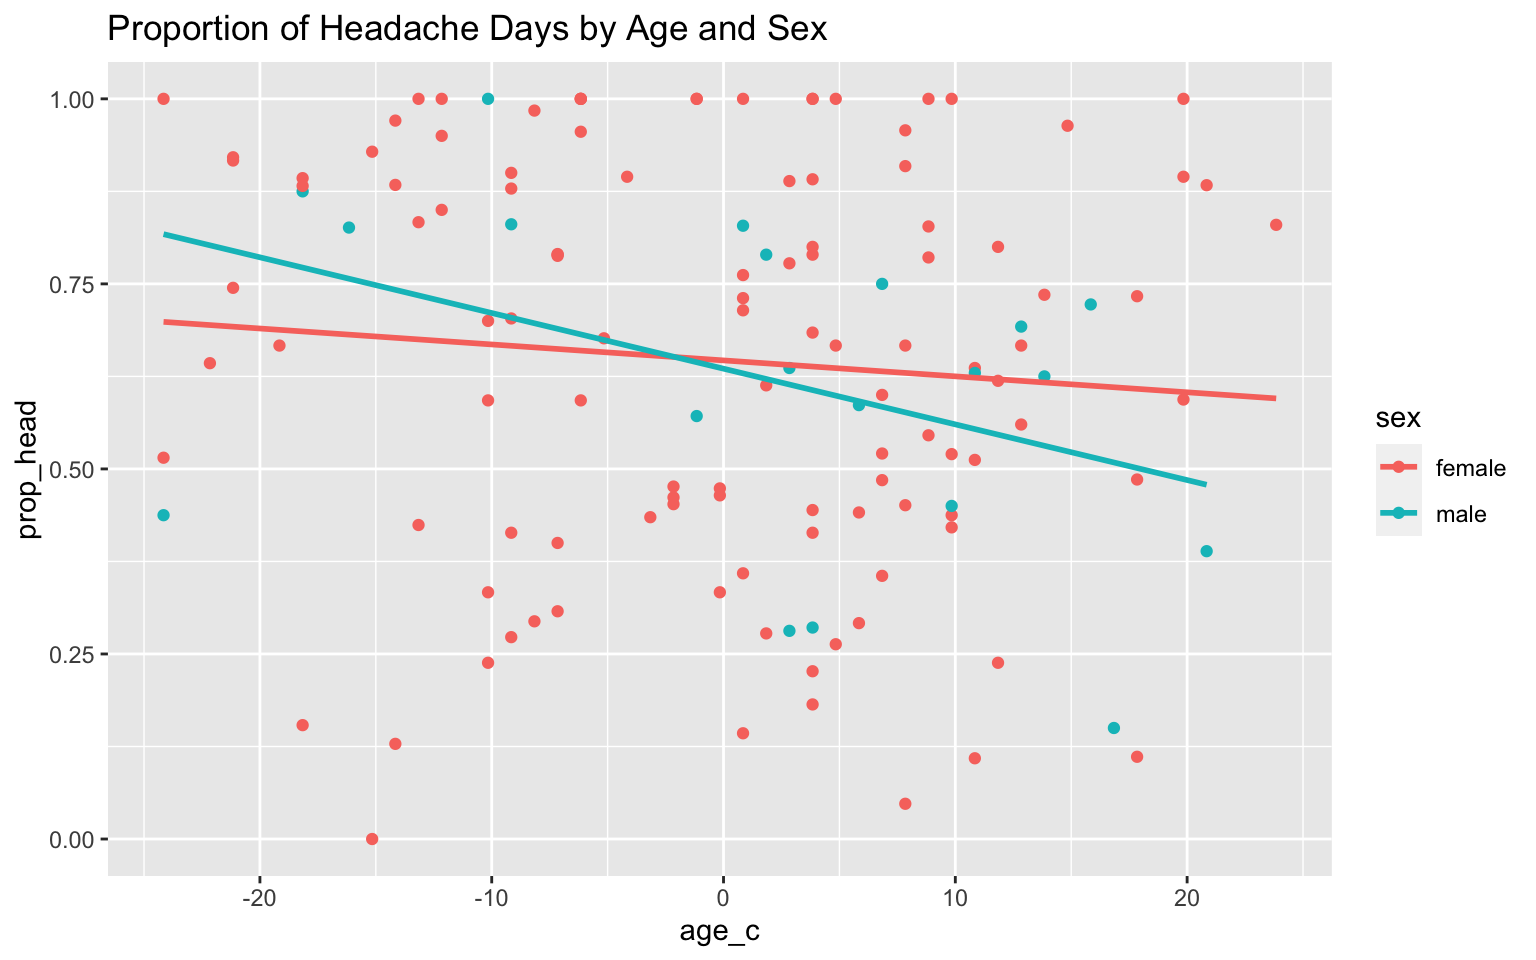
\includegraphics{project2final_files/figure-latex/unnamed-chunk-12-1} \end{center}

Going back, the assumptions of linearity, normality, and
homoskedasticity need to be checked prior to interpreting these results
with any confidence.

\begin{itemize}
\tightlist
\item
  \textbf{Linearity}:
\end{itemize}

\begin{Shaded}
\begin{Highlighting}[]
\KeywordTok{ggplot}\NormalTok{(headache2, }\KeywordTok{aes}\NormalTok{(age_c, prop_head)) }\OperatorTok{+}\StringTok{ }\KeywordTok{geom_point}\NormalTok{() }\OperatorTok{+}\StringTok{ }
\StringTok{  }\KeywordTok{ggtitle}\NormalTok{(}\StringTok{"Proportion of Headache Days by Age"}\NormalTok{)}
\end{Highlighting}
\end{Shaded}

\begin{center}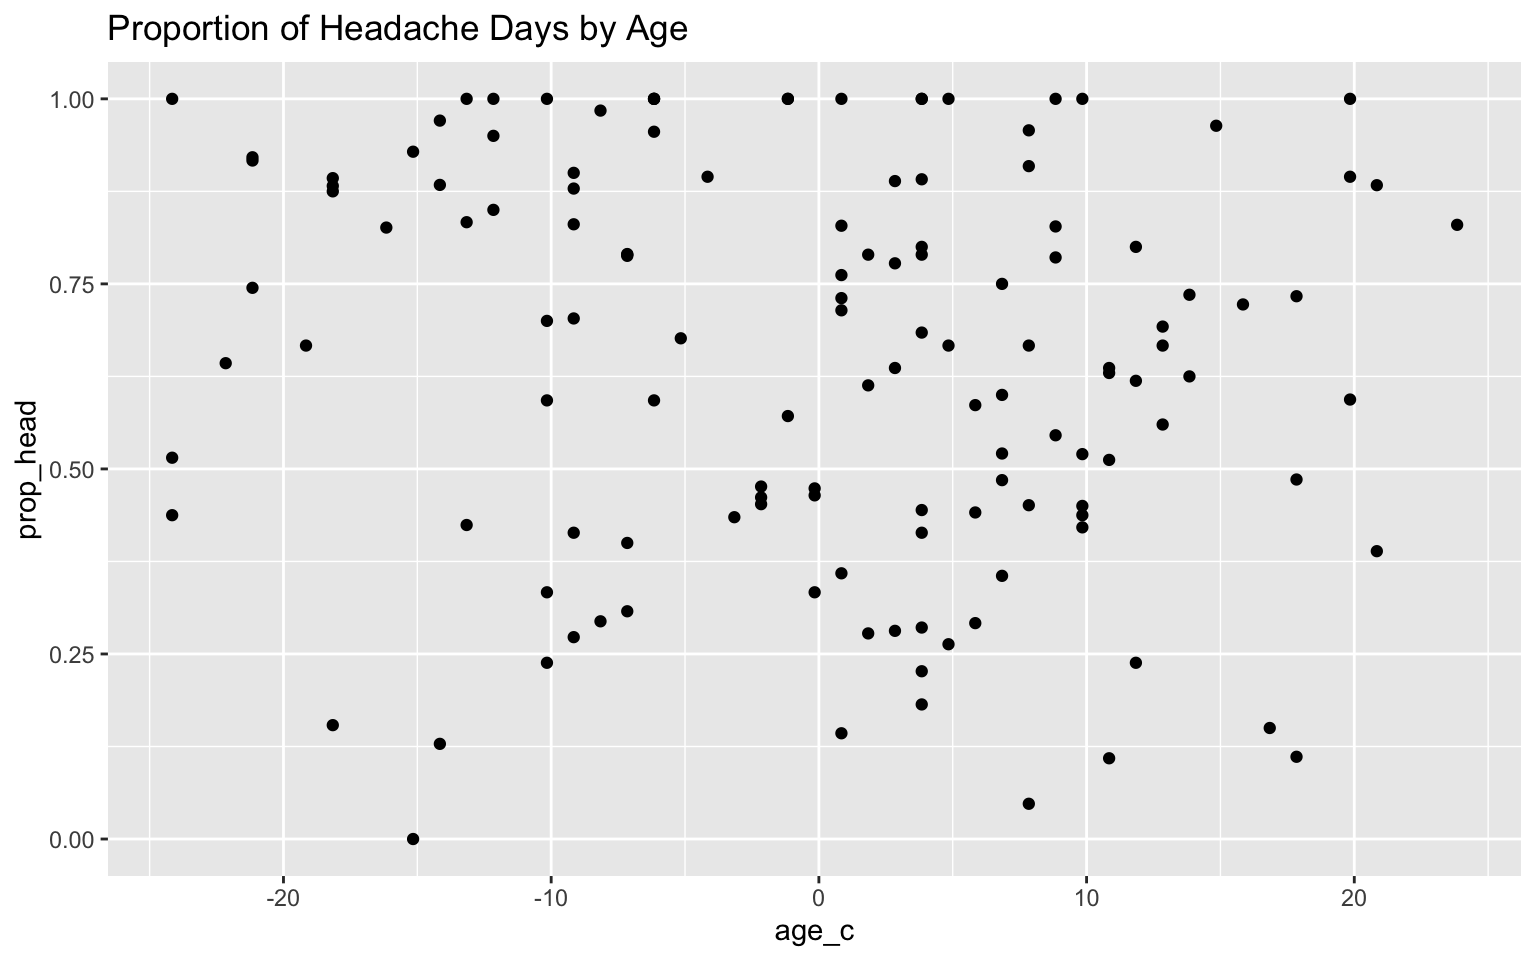
\includegraphics{project2final_files/figure-latex/unnamed-chunk-13-1} \end{center}

The linearity assumption is met, as there is no evidence of curves in
the scatterplot of age vs proportion of headaches. \(\checkmark\)

\begin{itemize}
\item
  \textbf{Normality}: The Shapiro-Wilk test was conducted to test the
  assumption of normality.

  \begin{itemize}
  \tightlist
  \item
    Ho: The distribution is normal
  \item
    HA: The distribution is not normal
  \end{itemize}
\end{itemize}

\begin{Shaded}
\begin{Highlighting}[]
\NormalTok{resids <-}\StringTok{ }\NormalTok{fit1}\OperatorTok{$}\NormalTok{residuals}
\KeywordTok{shapiro.test}\NormalTok{(resids)}
\end{Highlighting}
\end{Shaded}

\begin{verbatim}
## 
##  Shapiro-Wilk normality test
## 
## data:  resids
## W = 0.95246, p-value = 0.0001462
\end{verbatim}

The results of the Shapiro-Wilk test show that p\textless{}.001, so we
reject the null hypothesis and assume that the distribution is not
normal. Therefore, the assumption of normality is not passed.

\begin{itemize}
\tightlist
\item
  \textbf{Homodskedasticity}:
\end{itemize}

\begin{Shaded}
\begin{Highlighting}[]
\NormalTok{fitvals <-}\StringTok{ }\NormalTok{fit1}\OperatorTok{$}\NormalTok{fitted.values}
\KeywordTok{ggplot}\NormalTok{() }\OperatorTok{+}\StringTok{ }\KeywordTok{geom_point}\NormalTok{(}\KeywordTok{aes}\NormalTok{(fitvals, resids)) }\OperatorTok{+}\StringTok{ }\KeywordTok{geom_hline}\NormalTok{(}\DataTypeTok{yintercept=}\DecValTok{0}\NormalTok{)}
\end{Highlighting}
\end{Shaded}

\begin{center}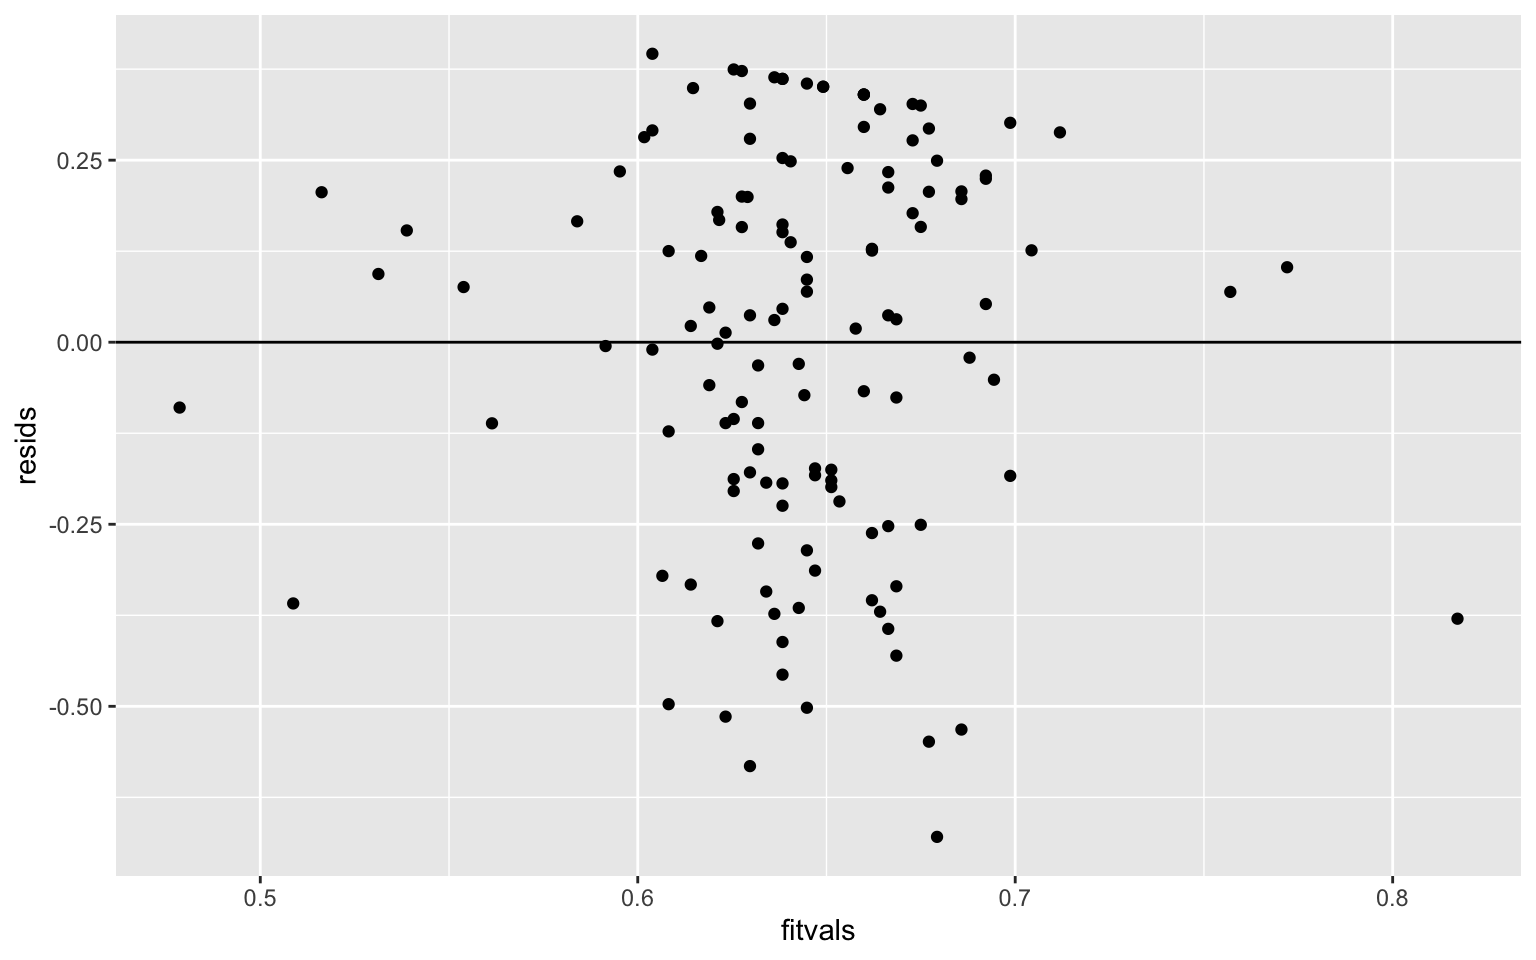
\includegraphics{project2final_files/figure-latex/unnamed-chunk-15-1} \end{center}

Though the variance of the residuals does not necessarily look equal
along the entirety of the line, there is no obvious fanning of the
points. Therefore, the assumption of homoskedasticity is met.
\(\checkmark\)

Even though the assumption of homoskedasticity was met, the regression
was recomputed with \textbf{robust standard errors}:

\begin{Shaded}
\begin{Highlighting}[]
\KeywordTok{library}\NormalTok{(sandwich)}
\KeywordTok{library}\NormalTok{(lmtest)}
\KeywordTok{coeftest}\NormalTok{(fit1, }\DataTypeTok{vcov=}\KeywordTok{vcovHC}\NormalTok{(fit1))}
\end{Highlighting}
\end{Shaded}

\begin{verbatim}
##
## t test of coefficients:
##
## Estimate Std. Error t value Pr(>|t|)
## (Intercept) 0.6466287 0.0261586 24.7195 <2e-16 ***
## age_c -0.0021548 0.0023850 -0.9035 0.3680
## sexmale -0.0112008 0.0631699 -0.1773 0.8595
## age_c:sexmale -0.0053685 0.0062781 -0.8551 0.3941
## ---
## Signif. codes: 0 '***' 0.001 '**' 0.01 '*' 0.05 '.' 0.1
' ' 1
\end{verbatim}

After recomputing with robust standard errors, there was not much change
seen in the regression results. The standard errors increased slightly
(except for ``sexmale'' that saw a slight decrease), and the p-values
followed this trend with a slight increase (except for ``sexmale'' which
slightly decreased). All p-values were much greater than .001, which
means they are not significant predictors for proportion of headache
days. Along with this, the coefficients remained relatively unchanged as
well. Looking at the \textbf{R-squared value}, we see that the
proportion of variation in the response variable that is explained by
the overall model is only .003097. This is an extremely low proportion,
signifying a weak model.

\#\#\#Bootstrapped Standard Errors Because the normality assumption was
not passed, the same regressin was run again with bootstrapped standard
errors:

\begin{Shaded}
\begin{Highlighting}[]
\NormalTok{headache2 <-}\StringTok{ }\NormalTok{headache2 }\OperatorTok\StringTok{ }\KeywordTok{ungroup}\NormalTok{() }\OperatorTok\StringTok{ }\KeywordTok{select}\NormalTok{(}\OperatorTok{-}\NormalTok{id)}

\KeywordTok{set.seed}\NormalTok{(}\DecValTok{1234}\NormalTok{)}
\NormalTok{samp_dist <-}\StringTok{ }\KeywordTok{replicate}\NormalTok{(}\DecValTok{5000}\NormalTok{, \{}
\NormalTok{boot <-}\StringTok{ }\KeywordTok{sample_frac}\NormalTok{(headache2, }\DataTypeTok{replace=}\NormalTok{T)}
\NormalTok{fit2 <-}\StringTok{ }\KeywordTok{lm}\NormalTok{(prop_head}\OperatorTok{~}\NormalTok{age_c}\OperatorTok{*}\NormalTok{sex, }\DataTypeTok{data=}\NormalTok{boot)}
\KeywordTok{coef}\NormalTok{(fit2)}
\NormalTok{\})}

\NormalTok{samp_dist }\OperatorTok\StringTok{ }\NormalTok{t }\OperatorTok\StringTok{ }\NormalTok{as.data.frame }\OperatorTok\StringTok{ }\KeywordTok{summarize_all}\NormalTok{(sd)}
\end{Highlighting}
\end{Shaded}

\begin{verbatim}
##   (Intercept)       age_c    sexmale age_c:sexmale
## 1  0.02563543 0.002345111 0.05633295   0.005252499
\end{verbatim}

With bootstrapping the standard errors, the standard errors for all
variables decreased very slightly, though these changes are almost
negligable amounts. The change observed is the same for both the
original model and the robust standard error model, as they both had
relatively the same values. Because all of the standard errors slightly
decreased, this means all of the p-values should also slightly decrease
from their values in the original model.

\#\#\#Logistic Regression Next, a logistic regression was run to
determine how days since onset of treatment and whether the medication
is being continued, reduced, or discontinued can predict whether the
patient had a headache or not. This might be important in seeing how the
length of time that treatment was administered or the level of the
treatment can predict the response of headache occurances in patients.
First, the ``headache'' variable was converted into a binary. Then, the
regression was run.

\begin{Shaded}
\begin{Highlighting}[]
\NormalTok{headache4 <-}\StringTok{ }\NormalTok{headache }\OperatorTok\StringTok{ }\KeywordTok{mutate}\NormalTok{(}\DataTypeTok{headache_occur=}\KeywordTok{ifelse}\NormalTok{(headache}\OperatorTok{==}\StringTok{"yes"}\NormalTok{,}\DecValTok{1}\NormalTok{,}\DecValTok{0}\NormalTok{)) }\OperatorTok\StringTok{ }
\StringTok{  }\KeywordTok{select}\NormalTok{(headache_occur, time, medication)}
\NormalTok{headache4}\OperatorTok{$}\NormalTok{medication <-}\StringTok{ }\KeywordTok{factor}\NormalTok{(headache4}\OperatorTok{$}\NormalTok{medication, }\DataTypeTok{ordered =} \OtherTok{FALSE}\NormalTok{ )}
\NormalTok{headache4}\OperatorTok{$}\NormalTok{medication <-}\StringTok{ }\KeywordTok{relevel}\NormalTok{(headache4}\OperatorTok{$}\NormalTok{medication, }\DataTypeTok{ref=}\StringTok{"none"}\NormalTok{)}
\NormalTok{fit3 <-}\StringTok{ }\KeywordTok{glm}\NormalTok{(headache_occur}\OperatorTok{~}\NormalTok{time}\OperatorTok{+}\NormalTok{medication, }\DataTypeTok{data=}\NormalTok{headache4, }\DataTypeTok{family=}\StringTok{"binomial"}\NormalTok{)}
\KeywordTok{coeftest}\NormalTok{(fit3)}
\end{Highlighting}
\end{Shaded}

\begin{verbatim}
##
## z test of coefficients:
##
## Estimate Std. Error z value Pr(>|z|)
## (Intercept) -0.1456010 0.0778190 -1.8710 0.061342 .
## time -0.0052268 0.0015956 -3.2757 0.001054 **
## medicationcontinuing 0.8416751 0.0846877 9.9386 <
2.2e-16 ***
## medicationreduced 1.5100027 0.1057633 14.2772 < 2.2e-16
***
## ---
## Signif. codes: 0 '***' 0.001 '**' 0.01 '*' 0.05 '.' 0.1
' ' 1
\end{verbatim}

\begin{Shaded}
\begin{Highlighting}[]
\KeywordTok{coeftest}\NormalTok{(fit3) }\OperatorTok\StringTok{ }\NormalTok{exp}
\end{Highlighting}
\end{Shaded}

\begin{verbatim}
##
## z test of coefficients:
##
## Estimate Std. Error z value Pr(>|z|)
## (Intercept) 0.86450 1.08093 1.5400e-01 1.063
## time 0.99479 1.00160 3.7800e-02 1.001
## medicationcontinuing 2.32025 1.08838 2.0714e+04 1.000
## medicationreduced 4.52674 1.11156 1.5867e+06 1.000
\end{verbatim}

The logistic regression resulted in the following coefficients: the
``intercept'' coefficient says that for someone who is experiencing at 0
days of treatment who is in the ``none'' group of treatment, the odds of
experiencing a headache is .86450; the ``time'' coefficient says that
for every 1 day increase in time, their odds of experiencing a headache
decreases and is .99479 times the odds for someone on day 0 of treatment
in the ``none'' group; the ``medicationcontinuing'' coefficient says
that for someone who will be continuing medication, their odds of
experiencing a headache increases and is 2.32025 times the odds for
someone who is not getting treatment; the ``medicationreduced''
coefficient says that for someone who has reduced medication, their odds
of experiencing a headache increases and is 4.52674 times higher than
someone who is continuing treatment.

A \textbf{confusion matrix}, comparing the true headache occurance
versus the predicted headache occurance, can be shown by:

\begin{Shaded}
\begin{Highlighting}[]
\NormalTok{prob <-}\StringTok{ }\KeywordTok{predict}\NormalTok{(fit3, }\DataTypeTok{type =} \StringTok{"response"}\NormalTok{)}
\NormalTok{pred <-}\StringTok{ }\KeywordTok{ifelse}\NormalTok{(prob }\OperatorTok{>}\StringTok{ }\FloatTok{0.5}\NormalTok{, }\DecValTok{1}\NormalTok{, }\DecValTok{0}\NormalTok{)}
\KeywordTok{table}\NormalTok{(}\DataTypeTok{prediction =}\NormalTok{ pred, }\DataTypeTok{truth =}\NormalTok{ headache4}\OperatorTok{$}\NormalTok{headache_occur) }\OperatorTok\StringTok{ }\NormalTok{addmargins}
\end{Highlighting}
\end{Shaded}

\begin{verbatim}
##           truth
## prediction    0    1  Sum
##        0    440  343  783
##        1   1046 2323 3369
##        Sum 1486 2666 4152
\end{verbatim}

Based on this confusion matrix, the model predicted 2323 true positives,
440 true negatives, 343 false negatives, and 1046 false positives. The
extremely high false positive rate signifies that this model
overpredicts headache occurance, when in reality a lot of these patients
did not experience headaches. This can be further analyzed through:

\begin{Shaded}
\begin{Highlighting}[]
\CommentTok{#accuracy:}
\NormalTok{(}\DecValTok{440}\OperatorTok{+}\DecValTok{2323}\NormalTok{)}\OperatorTok{/}\DecValTok{4152}
\end{Highlighting}
\end{Shaded}

\begin{verbatim}
## [1] 0.6654624
\end{verbatim}

\begin{Shaded}
\begin{Highlighting}[]
\CommentTok{#sensitivity(TPR):}
\NormalTok{(}\DecValTok{2323}\NormalTok{)}\OperatorTok{/}\DecValTok{2666}
\end{Highlighting}
\end{Shaded}

\begin{verbatim}
## [1] 0.8713428
\end{verbatim}

\begin{Shaded}
\begin{Highlighting}[]
\CommentTok{#specificity(TNR):}
\NormalTok{(}\DecValTok{440}\NormalTok{)}\OperatorTok{/}\DecValTok{1486}
\end{Highlighting}
\end{Shaded}

\begin{verbatim}
## [1] 0.2960969
\end{verbatim}

\begin{Shaded}
\begin{Highlighting}[]
\CommentTok{#Recall(PPV):}
\NormalTok{(}\DecValTok{2323}\NormalTok{)}\OperatorTok{/}\DecValTok{3369}
\end{Highlighting}
\end{Shaded}

\begin{verbatim}
## [1] 0.6895221
\end{verbatim}

The \textbf{accuracy} rate, or the proportion of predictions that
correctly depicted reality, is fairly high at .6654624. The
\textbf{sensitivity}, or the proportion of headache occurances that were
correctly predicted to be headache occurances, is also pretty high at
.8713428. However, the \textbf{specificity}, or the proportion of
non-headache occurances correctly classified as non-headache occurances,
was low at only .2960969. The \textbf{recall}, or proportion of the
classified headache occurances that actually were headache occurances,
was a fair proportion at .6895221. Though the model is not very good at
predicting with specificity, it is much stronger at predicting with
sensitivity. These strengths and weaknesses balance out when we look at
the average overall accuracy (we see the trade-offs!).

The \textbf{density of log-odds} (logit) by headache occurance can be
shown by:

\begin{Shaded}
\begin{Highlighting}[]
\NormalTok{headache4}\OperatorTok{$}\NormalTok{logit <-}\StringTok{ }\KeywordTok{predict}\NormalTok{(fit3, }\DataTypeTok{type=}\StringTok{"link"}\NormalTok{)}
\NormalTok{headache4 }\OperatorTok\StringTok{ }\KeywordTok{ggplot}\NormalTok{(}\KeywordTok{aes}\NormalTok{(logit, }\DataTypeTok{fill=}\KeywordTok{factor}\NormalTok{(headache_occur))) }\OperatorTok{+}
\StringTok{  }\KeywordTok{geom_density}\NormalTok{(}\DataTypeTok{alpha=}\NormalTok{.}\DecValTok{3}\NormalTok{) }\OperatorTok{+}\StringTok{ }\KeywordTok{geom_vline}\NormalTok{(}\DataTypeTok{xintercept=}\DecValTok{0}\NormalTok{, }\DataTypeTok{color=}\StringTok{'red'}\NormalTok{) }\OperatorTok{+}
\StringTok{  }\KeywordTok{labs}\NormalTok{(}\DataTypeTok{fill=}\StringTok{"headache"}\NormalTok{)}
\end{Highlighting}
\end{Shaded}

\begin{center}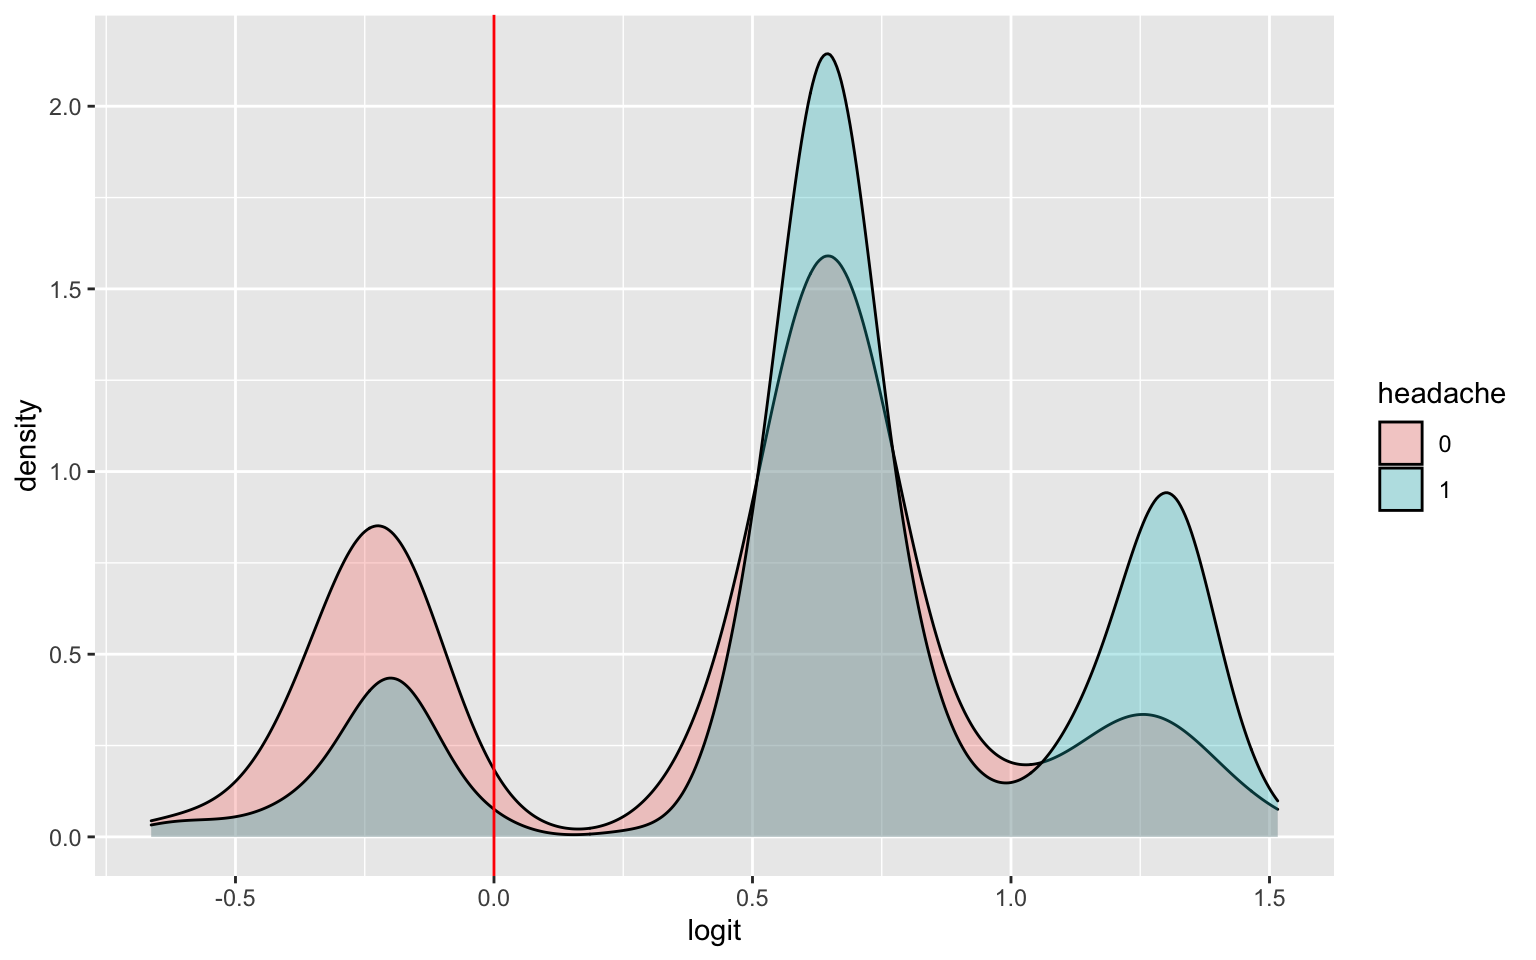
\includegraphics{project2final_files/figure-latex/unnamed-chunk-21-1} \end{center}

From this plot, the rates described above are illustrated. The high
sensitivity is demonstrated by the high blue peaks above the logit=0
line, as this indicates true headache occurances that were predicted to
be headache occurances. The low specificity is shown by the low pink
peak below the logit=0 line, as this indicates that not many of the true
non-headache occurances were classified as such. The average value for
recall is seen by the fact that though there are a lot of correctly
classified headache occurances (blue peaks to the right of the logit=0
line), there is still a significant number of non-headache occurances
that were classified as headaches (pink peaks to the right of the
logit=0 line). The grey ``overlapped density'' areas represent logit
values where both true headache occurances and non-headache occurances
happen, therefore areas where logit is not a good predictor to
differentiate between the two headache groups.

Another way to represent these rates is with an \textbf{ROC curve} and
\textbf{AUC} calculation:

\begin{Shaded}
\begin{Highlighting}[]
\KeywordTok{library}\NormalTok{(plotROC)}
\NormalTok{headache4}\OperatorTok{$}\NormalTok{prob<-}\KeywordTok{predict}\NormalTok{(fit3,}\DataTypeTok{type=}\StringTok{"response"}\NormalTok{)}
\NormalTok{ROC <-}\StringTok{ }\KeywordTok{ggplot}\NormalTok{(headache4) }\OperatorTok{+}\StringTok{ }\KeywordTok{geom_roc}\NormalTok{(}\KeywordTok{aes}\NormalTok{(}\DataTypeTok{d=}\NormalTok{headache_occur, }\DataTypeTok{m=}\NormalTok{prob), }\DataTypeTok{n.cuts=}\DecValTok{0}\NormalTok{)}
\NormalTok{ROC}
\end{Highlighting}
\end{Shaded}

\begin{center}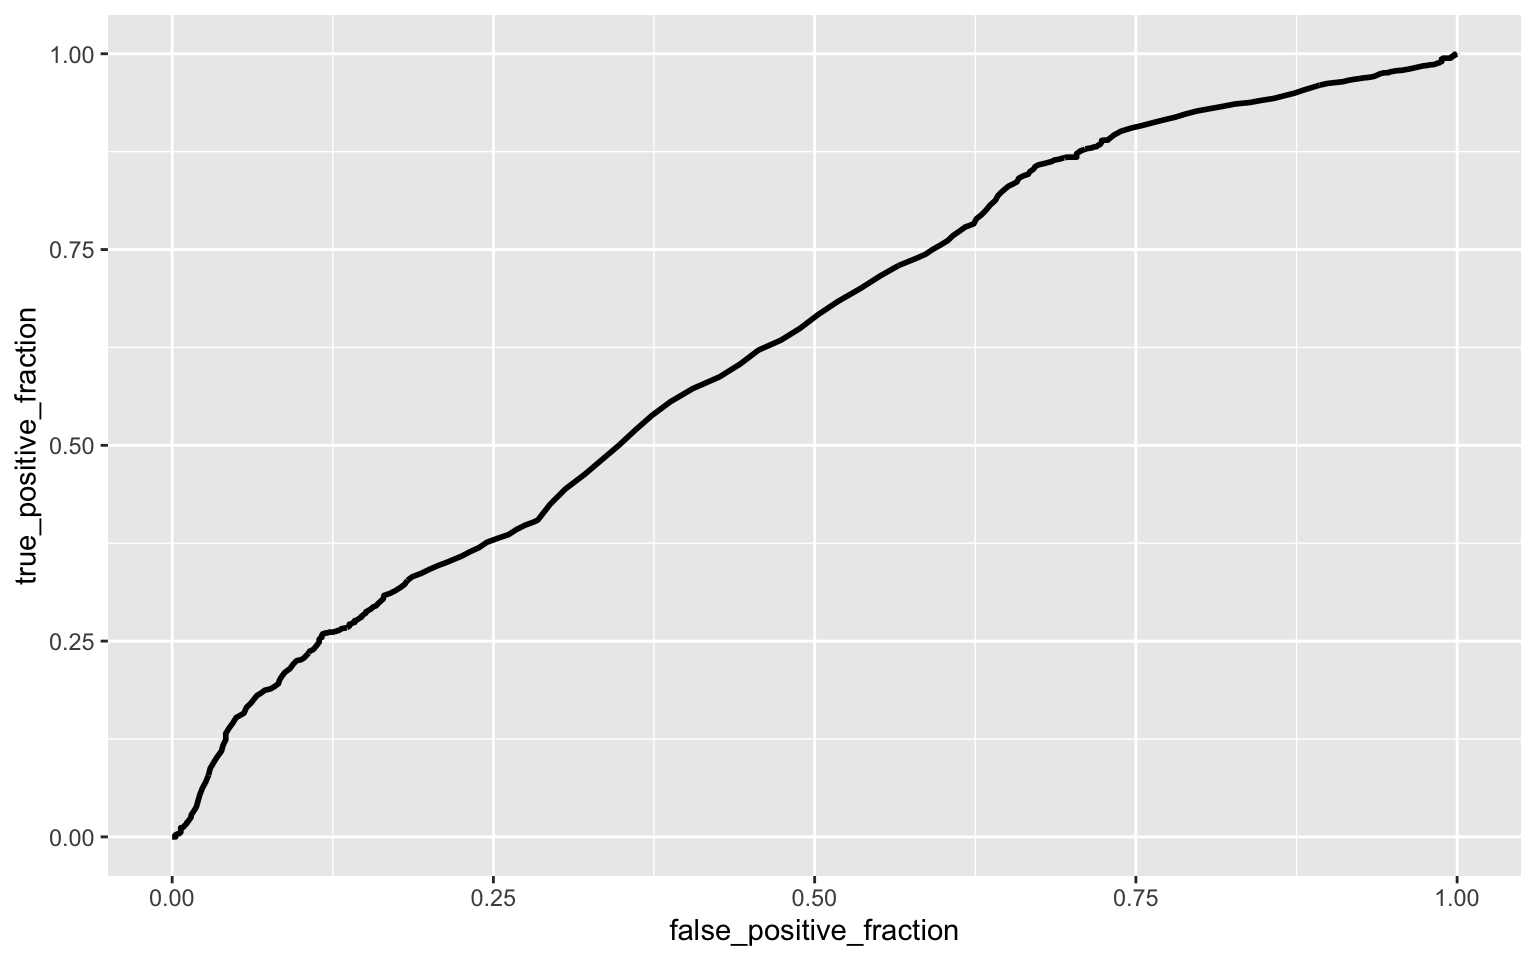
\includegraphics{project2final_files/figure-latex/unnamed-chunk-22-1} \end{center}

\begin{Shaded}
\begin{Highlighting}[]
\KeywordTok{calc_auc}\NormalTok{(ROC)}
\end{Highlighting}
\end{Shaded}

\begin{verbatim}
##   PANEL group       AUC
## 1     1    -1 0.6271121
\end{verbatim}

The ROC curve shows us the relationship between false positives and true
positives as we change the cutoff value for the model. Ideally, the true
positive rate would stay high even as we increase the false positive
rate, resulting in an AUC value of 1. The AUC value we calculated of
.6271121 tells us that the model is a poor predictor of headache
occurance. This weakness is demonstrated by the shape of the ROC curve,
as the true positive rate remains relatively low for a while even as the
false positive rate increases. Though the model is poor, it might not be
completely useless as the AUC value is above a value of .5, which would
mean the model predicts no better than choosing a response at random.

\textbf{Cross-validation} can be used on this model to see how it can be
applied to other data other than that which was used to produce the
model:

\begin{Shaded}
\begin{Highlighting}[]
\KeywordTok{set.seed}\NormalTok{(}\DecValTok{1234}\NormalTok{)}
\NormalTok{k=}\DecValTok{10}

\NormalTok{data <-}\StringTok{ }\NormalTok{headache4[}\KeywordTok{sample}\NormalTok{(}\KeywordTok{nrow}\NormalTok{(headache4)),]}
\NormalTok{fold <-}\StringTok{ }\KeywordTok{cut}\NormalTok{(}\KeywordTok{seq}\NormalTok{(}\DecValTok{1}\OperatorTok{:}\KeywordTok{nrow}\NormalTok{(headache4)), }\DataTypeTok{breaks=}\NormalTok{k, }\DataTypeTok{labels=}\NormalTok{F)}
\NormalTok{val <-}\StringTok{ }\OtherTok{NULL}
\ControlFlowTok{for}\NormalTok{(i }\ControlFlowTok{in} \DecValTok{1}\OperatorTok{:}\NormalTok{k)\{}
\NormalTok{  trainset <-}\StringTok{ }\NormalTok{data[fold}\OperatorTok{!=}\NormalTok{i,]}
\NormalTok{  testset <-}\StringTok{ }\NormalTok{data[fold}\OperatorTok{==}\NormalTok{i,]}
\NormalTok{  truth <-}\StringTok{ }\NormalTok{testset}\OperatorTok{$}\NormalTok{headache_occur}
\NormalTok{  fit4 <-}\StringTok{ }\KeywordTok{glm}\NormalTok{(headache_occur}\OperatorTok{~}\NormalTok{medication}\OperatorTok{+}\NormalTok{time, }\DataTypeTok{data=}\NormalTok{trainset, }\DataTypeTok{family=}\StringTok{"binomial"}\NormalTok{)}
\NormalTok{  prob <-}\StringTok{ }\KeywordTok{predict}\NormalTok{(fit4, }\DataTypeTok{newdata=}\NormalTok{testset, }\DataTypeTok{type=}\StringTok{"response"}\NormalTok{)}
\NormalTok{  val <-}\StringTok{ }\KeywordTok{rbind}\NormalTok{(val, }\KeywordTok{class_diag}\NormalTok{(prob, truth))}
\NormalTok{\}}
\KeywordTok{summarize_all}\NormalTok{(val, mean)}
\end{Highlighting}
\end{Shaded}

\begin{verbatim}
##         acc      sens      spec       ppv       auc
## 1 0.6659546 0.8723044 0.2952242 0.6895378 0.6273299
\end{verbatim}

After a 10-fold cross-validation, the AUC remains about the same at
.6265165. The average out-of-sample accuracy is .6652352, while the
sensitivity is .8714029 and the recall is .6893232. These values only
vary slightly from the full-model values.

\#\#\#LASSO Focusing only on Aura and non-Aura headaches (excluding the
``mixed'' headache patients), a LASSO regression was run to see which
variables best predict the type of headache that the patient
experiences. These results could tell us what factors best predict a
future patient's probability of having aura headaches as opposed to
non-aura headaches.

\begin{Shaded}
\begin{Highlighting}[]
\KeywordTok{library}\NormalTok{(glmnet)}
\NormalTok{headache5 <-}\StringTok{ }\NormalTok{headache }\OperatorTok\StringTok{ }\KeywordTok{select}\NormalTok{(}\OperatorTok{-}\NormalTok{id) }\OperatorTok\StringTok{ }\KeywordTok{filter}\NormalTok{(hatype}\OperatorTok{!=}\StringTok{"Mixed"}\NormalTok{)}
\NormalTok{y <-}\StringTok{ }\KeywordTok{as.matrix}\NormalTok{(headache5}\OperatorTok{$}\NormalTok{hatype)}
\NormalTok{x <-}\StringTok{ }\KeywordTok{model.matrix}\NormalTok{(hatype}\OperatorTok{~}\NormalTok{., }\DataTypeTok{data=}\NormalTok{headache5)[,}\OperatorTok{-}\DecValTok{1}\NormalTok{]}
\KeywordTok{head}\NormalTok{(x)}
\end{Highlighting}
\end{Shaded}

\begin{verbatim}
## time dos age airq medicationnone medicationreduced
headacheyes sexmale
## 1 -11 753 30 9 0 0 1 0
## 2 -10 754 30 7 0 0 1 0
## 3 -9 755 30 10 0 0 1 0
## 4 -8 756 30 13 0 0 1 0
## 5 -7 757 30 18 0 0 1 0
## 6 -6 758 30 19 0 0 1 0
\end{verbatim}

\begin{Shaded}
\begin{Highlighting}[]
\NormalTok{x <-}\StringTok{ }\KeywordTok{scale}\NormalTok{(x)}
\NormalTok{cv <-}\StringTok{ }\KeywordTok{cv.glmnet}\NormalTok{(x, y, }\DataTypeTok{family =} \StringTok{"binomial"}\NormalTok{)}
\NormalTok{lasso <-}\StringTok{ }\KeywordTok{glmnet}\NormalTok{(x, y, }\DataTypeTok{family =} \StringTok{"binomial"}\NormalTok{, }\DataTypeTok{lambda =}\NormalTok{ cv}\OperatorTok{$}\NormalTok{lambda}\FloatTok{.1}\NormalTok{se)}
\KeywordTok{coef}\NormalTok{(lasso)}
\end{Highlighting}
\end{Shaded}

\begin{verbatim}
## 9 x 1 sparse Matrix of class "dgCMatrix"
##                            s0
## (Intercept)        0.16129030
## time               .         
## dos                0.29161978
## age                0.21255913
## airq               0.14476652
## medicationnone    -0.03325123
## medicationreduced  0.24532956
## headacheyes       -0.10319022
## sexmale            0.17380451
\end{verbatim}

Based on the LASSO regression, using ``lambda.1se'' in order to maximize
regularization, all variables were retained except for ``time''. This
means that in order to maximize the strength of the model as a predictor
without overfitting to the current data, ``time'' should be excluded.
This can be further analyzed through a \textbf{10-fold
cross-validation}:

\begin{Shaded}
\begin{Highlighting}[]
\NormalTok{headache6 <-}\StringTok{ }\NormalTok{headache5 }\OperatorTok\StringTok{ }\KeywordTok{select}\NormalTok{(}\OperatorTok{-}\NormalTok{time) }\OperatorTok\StringTok{ }\KeywordTok{mutate}\NormalTok{(}\DataTypeTok{hatype=}\KeywordTok{ifelse}\NormalTok{(hatype}\OperatorTok{==}\StringTok{"Aura"}\NormalTok{,}\DecValTok{1}\NormalTok{,}\DecValTok{0}\NormalTok{))}
\KeywordTok{set.seed}\NormalTok{(}\DecValTok{1234}\NormalTok{)}
\NormalTok{k=}\DecValTok{10}
\NormalTok{data2 <-}\StringTok{ }\NormalTok{headache6 }\OperatorTok\StringTok{ }\NormalTok{sample_frac}
\NormalTok{folds2 <-}\StringTok{ }\KeywordTok{ntile}\NormalTok{(}\DecValTok{1}\OperatorTok{:}\KeywordTok{nrow}\NormalTok{(data2), }\DataTypeTok{n=}\DecValTok{10}\NormalTok{)}
\NormalTok{val2 <-}\StringTok{ }\OtherTok{NULL}
\ControlFlowTok{for}\NormalTok{(i }\ControlFlowTok{in} \DecValTok{1}\OperatorTok{:}\NormalTok{k)\{}
\NormalTok{  trainset2 <-}\StringTok{ }\NormalTok{data2[folds2}\OperatorTok{!=}\NormalTok{i,]}
\NormalTok{  testset2 <-}\StringTok{ }\NormalTok{data2[folds2}\OperatorTok{==}\NormalTok{i,]}
\NormalTok{  truth2 <-}\StringTok{ }\NormalTok{testset2}\OperatorTok{$}\NormalTok{hatype}
\NormalTok{  fit5 <-}\StringTok{ }\KeywordTok{glm}\NormalTok{(hatype}\OperatorTok{~}\NormalTok{., }\DataTypeTok{data=}\NormalTok{trainset2, }\DataTypeTok{family=}\StringTok{"binomial"}\NormalTok{)}
\NormalTok{  prob2 <-}\StringTok{ }\KeywordTok{predict}\NormalTok{(fit5, }\DataTypeTok{newdata=}\NormalTok{testset2, }\DataTypeTok{type=}\StringTok{"response"}\NormalTok{)}
\NormalTok{  val2 <-}\StringTok{ }\KeywordTok{rbind}\NormalTok{(val2, }\KeywordTok{class_diag}\NormalTok{(prob2, truth2))}
\NormalTok{\}}
\NormalTok{val2 }\OperatorTok\StringTok{ }\KeywordTok{summarize_all}\NormalTok{(mean)}
\end{Highlighting}
\end{Shaded}

\begin{verbatim}
##         acc     sens      spec      ppv      auc
## 1 0.6013763 0.550073 0.6470447 0.573028 0.670824
\end{verbatim}

The out-of-sample accuracy for this regression is .2511389. This is much
lower than the accuracy of the previous logistic regression which was
.6652352 (note however that we are predicting a difference response
here). Though these variables were chosen as the best predictors for the
model based on what the model was provided, the variables themselves
might still not be significant predictors of headache type in real life
and therefore the low accuracy.

\#\#\#Summary Overall, these tests analyzed differences between headache
occurances and types in different demographics. These tools might be
helpful in diagnosing the type of headache or frequency of headaches
that someone is prone to based on factors such as age or airquality. The
MANOVA, ANOVA, and post-hoc tests found that for all headache types, the
average airquality differed significantly while the average age differed
significantly for all headache types except for when comparing ``mixed''
headaches and ``aura'' headaches. The randomization test focused in on
average airquality for when people experienced headaches versus when
they did not, and it was found that there was no significant difference
between airquality average values during headache occurance versus when
a headache was not experienced. The linear regression found that though
age and sex were not necessarily significant predictors of proportion of
headache days, 1 year increases and being male both predicted decreased
proportion of headache days in comparison to females of average age. The
logistic regression found that both days since the onset of treatment
and the level of treatment administered were both significant predictors
of headache occurance! The occurance of a headache was predicted to
increase significantly for patients who continued or reduced treament,
while the occurance of headache was predicted to decrease with increased
treatment time. Further clinical tests could be conducted based on this
result to determine if the changes in headache occurance was due to the
change in medicine level (if headache occurance had a predicted decrease
without treatment because the treatment was detrimental), or if the
medicine level was changed due to a change in headache occurance (if
headache occurance had a prediced decrease without treatment because
headache occurance lowered and therefore treatment was stopped).

Though many of the variables tested did not end up being significant
predictors of headache occurance, research that does not support a
theory can still be valuable! Further tests can be shaped on a lack of
significance, as knowledge that age or aiquality for example do not
cause someone to be prone to increased proportions of headaches can be
helpful in the development of treatment plans. \ldots{}

\end{document}
